\chapter{FEA data management}

Together with growing complexity of finite element calculations, the importance of management of data produced by the calculations is increasingly emphasized in both industrial and research communities. Information is often shared between multiple users, moved from one computer to another, and further transformed to enable different views over the data. Some definition of persistent and standard representation of the data is therefore required as well as the corresponding data access system architecture that allows to query the data.

\section{Data management system architecture}

The prototype implementation of the FEA data management system is designed as a collaborative framework that can be accessed by users from different client devices. Figure \ref{fig:FEA-architecture} depicts the schema of the system architecture. The system consists of several independent modules. The FEM calculation itself runs on a remote server as one of services along with a mesh generation service, a results processing service, etc. These services are controlled by an application service that provides interface to client applications in form of REST API.

\begin{figure}[H]
    \centering
    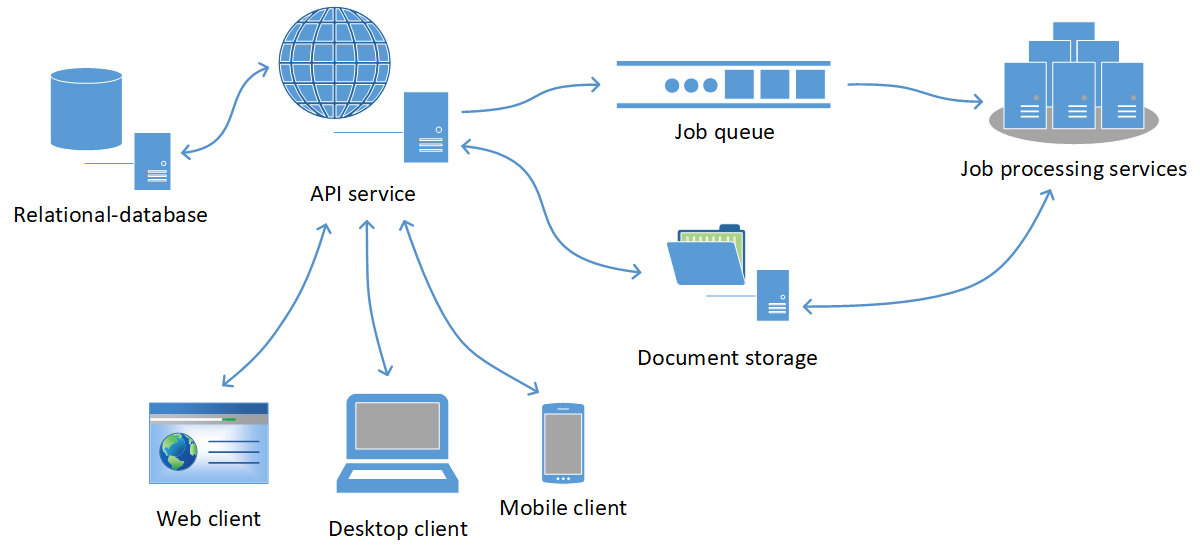
\includegraphics[width=\textwidth]{figures/chapter-data-management/FEA-architecture}
    \decoRule
    \caption{FEA system architecture.}
    \label{fig:FEA-architecture}
\end{figure}

The system contains two types of data storage. The relational-database type of storage is intended to store basic project-related data such as description of simulations, links to the simulation resources, information about the owner and other colaborating users, etc. The input to FEA -- geometrical model, attribute assignments, and analysis parameters -- can also be stored in a relational database, eventhough, storing this complex type of information in the SQL database is questionable and has its drawbacks.

The second type of storage is the blob storage used to hold temporary files being the input or the output of particular components, especially the mesh generator and the FEM solver. The system is designed to be independent of the solver and mesh generator components, therefore this intermediate step of converting the input to proprietary file format that the components understand is necessary. In the future, it is possible to expect a gradual transition from the file-based approach to the direct connection to the database and query the input model directly. Also, the output of the calculation could be saved directly in the proposed format to represent the results in post-process-ready form.

Workflow diagram in Figure \ref{fig:FEA-workflow} helps to visualize the sequence of FEA steps and the transfer of data between the service components. The vertical bars denote computational intensive tasks performed by the service components. The client side in the diagram represents the presentation layer of the FEA system that the user directly interacts with. In the presentation layer, also called \textit{frontend}, there is spent the vast majority of time by users doing pre- and post-processing of data (which is not depicted in the diagram). The web API service, also called \textit{backend}, is the key component that assigns work to other components. It serves as an controller for a running analysis and as an interface between the data stored in databases and the client applications.

\begin{figure}[H]
    \centering
    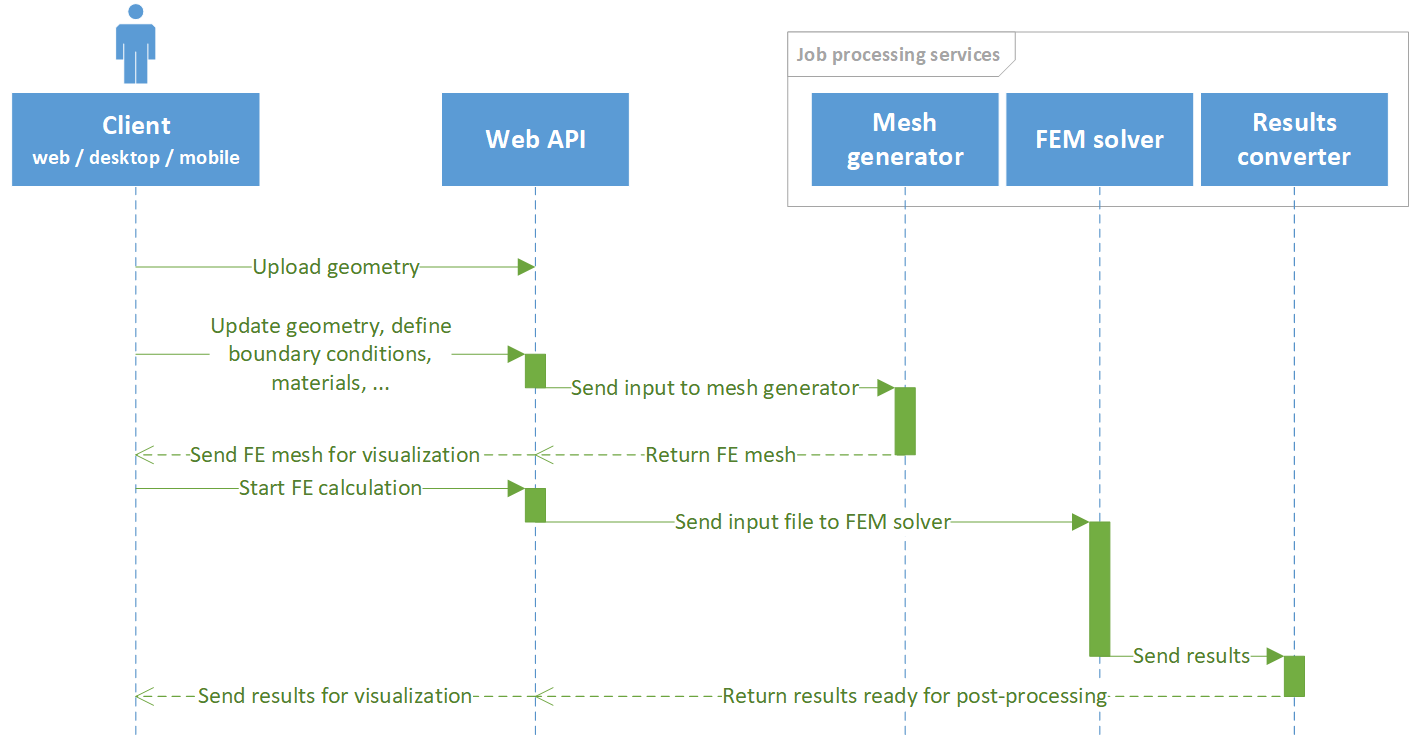
\includegraphics[width=\textwidth]{figures/chapter-data-management/FEA-workflow}
    \decoRule
    \caption{FEA system workflow.}
    \label{fig:FEA-workflow}
\end{figure}

The prototype implementation of the data management system follows the schema and the workflow depicted in Figures \ref{fig:FEA-architecture} and \ref{fig:FEA-workflow}. The difference is that the pre-processing phase is currently excluded. The focus of the work presented in the thesis is primarily on the post-processing features and the representation of results. Therefore, the results from the existing FEM solver are uploaded into the system and the system converts them to the internal representation suitable for post-processing. To test the prototype implementation of the data management system, two client applications are created. The first is the feature-rich desktop post-processor with the support for Linux and Windows operating systems. The second is the simple web application that provides basic control over an analysis and basic post-processing capabilities. Its purpose is mainly to demonstrate the benefits of proposed format for storage of results when post-processing complex FEA. Its web-based implementation allows for truly cross-platform experience without the need for installation and it allows to access the analysis data even from low-end mobile devices.


\section{Storage format for results}
\label{sec:storage-format}

The project-based data model with the representation of simulation results is depicted in Figure \ref{fig:FEA-db-schema-results} as ER diagram.

\begin{figure}[H]
    \centering
    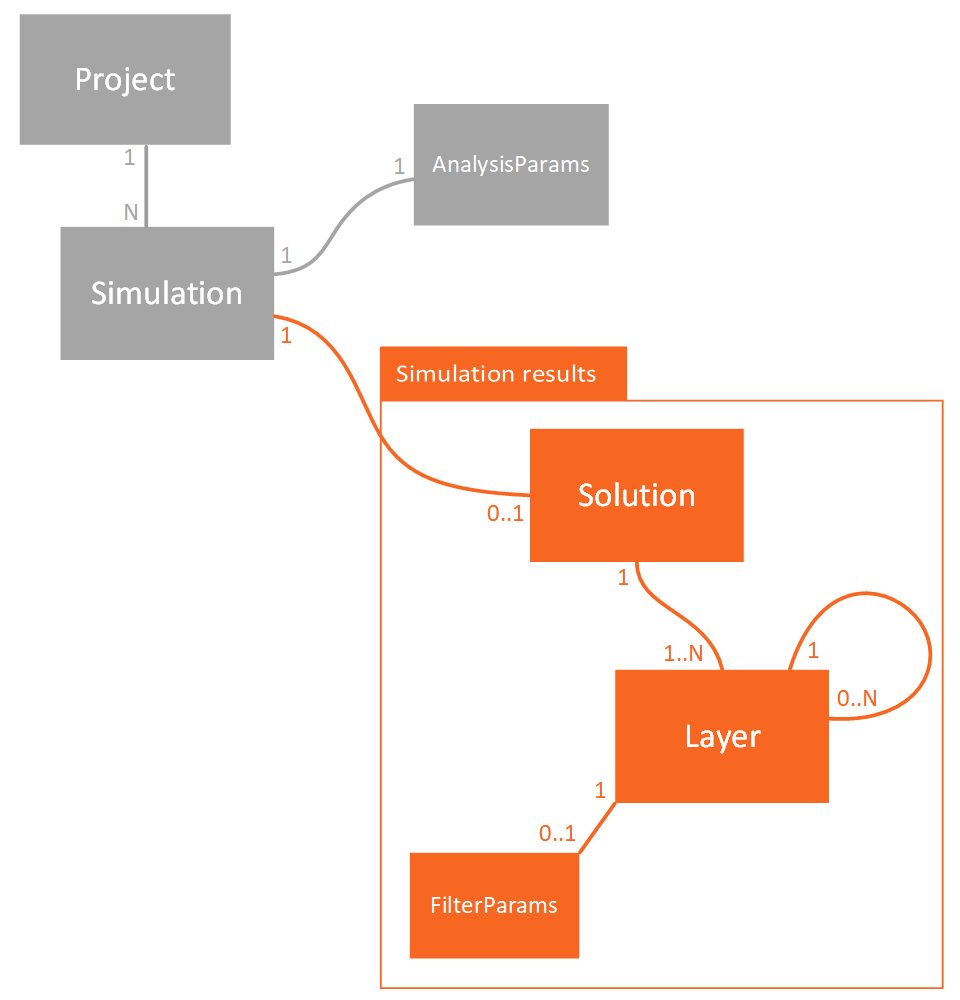
\includegraphics[width=0.8\textwidth]{figures/chapter-data-management/FEA-database-schema-only-results}
    \decoRule
    \caption[Database schema for FEA with results representation only.]{Database schema for FEA with results representation only (without the input model).}
    \label{fig:FEA-db-schema-results}
\end{figure}

The simulation results are represented by the Solution entity, which holds a structure consisting of the results from the FEM solver that are converted to the form suitable for post-processing. The structure has the form of a tree. A node of the tree is represented by the Layer entity. A layer is an association of a mesh and corresponding result fields and other attributes. The use of a tree structure allows to preserve the relations between the parent layers and the layers that are derived from them. The mesh that is referenced by a layer need not be the same as the mesh used as the input mesh to the FEM solver. It could be modified by the solver during the calculation, e.g., due to the use of adaptive finite element techniques. Also, the resulting mesh can be further modified to facilitate the post-processor implementation, e.g., a deformed mesh that helps to visualize the displacement results can be generated, or a number of cross-sections can be created at uniform intervals to provide a look on results inside the mesh. Generally, multiple views on the results can be prepared in advance before the user even starts to investigate the results.

The concept of layer is not new. It is used in existing implementations of the post-processors in FEA software packages (often named \textit{filter} instead of layer), to represent a view on the results. However, the layers (visual filters) are usually generated on demand by specific user request and they are not kept in a persistent storage. The proposed storage format for results is built on top of the layer tree structure directly, which allows the layers to be accessed later on, even on a different device, or shared by multiple users working on the same project.


\subsection{Format specification}

The key part of the format is the solution document. An example of the solution document is given in Listing \ref{lst:solution.json}. In case of remote storage, the solution document is stored in a relational database as part of the project-based data representation shown in Figure \ref{fig:FEA-db-schema-results}, while the rest of documents is stored in a blob storage as group of JSON documents. In case of local storage, all documents, including the solution document, are stored in a folder as JSON files in local file system on a personal computer on which the results are post-processed.

\begin{lstlisting}[style=json,caption=Example of solution.json document.,label=lst:solution.json]
    {
        "Id": 42,
        "ProjectName": "Shear beam 3D",
        "Location": "https://fea-cloud-service.net/postprocess/42",
        "Results": [
          {
            "MeshRecordNames": [
              "beam.msh"
            ],
            "DataRecordNames": [
              "beam.res"
            ]
          }
        ],
        "Layers": [
          {
            "Id": "5b585758-9f64-4790-a765-64709951931a",
            "Name": "master",
            "FilterType": null,
            "Children": [
              {
                "Id": "09dfdc8c-a75b-48e1-b319-a9624312a5a5",
                "Name": "deformation (scale: 0.6)",
                "FilterType": "Deformation",
                "Children": [
                  {
                    "Id": "ee52969e-f862-4daf-85b9-5a8224197669",
                    "Name": "slice (offset: -0.1569261)",
                    "FilterType": "Slice"
                  },
                  {
                    "Id": "a86486b1-53eb-43cc-aa22-d670bcdea163",
                    "Name": "slice (offset: -0.4757478)",
                    "FilterType": "Slice"
                  },
                  {
                    "Id": "6c6c4b8a-2280-4b4b-a51f-fcd5149f1d94",
                    "Name": "slice (offset: -0.8751443)",
                    "FilterType": "Slice"
                  }
                ]
              },
              {
                "Id": "96ca950c-0767-4439-b57a-35384ea351a7",
                "Name": "isosurface DISPLACEMENTS/X(1) = -0.0001",
                "FilterType": "IsoSurface"
              },
              {
                "Id": "2a3c47be-2f06-48f5-adfd-30777aea092c",
                "Name": "isosurface DISPLACEMENTS/X(1) = -0.0003",
                "FilterType": "IsoSurface"
              },
              {
                "Id": "7e5f043b-9900-427e-8d38-839ff1b8e27c",
                "Name": "isosurface DISPLACEMENTS/X(1) = -0.0007",
                "FilterType": "IsoSurface"
              }
            ]
          }
        ]
    }
    \end{lstlisting}

Data in each layer are stored in four types of documents. All documents are identified by the layer id, which is a GUID (Globally Unique IDentifier), and by its index within the layer (except Summary document that does not need an index as it exist in one instance per layer).
\begin{itemize}

    \item \textbf{Summary document} contains all the descriptive information about a layer. An example of a summary document in JSON format is presented in Listing \ref{lst:summary.json}.
    
% TODO: pridat 2 vety k summary dokumentu

    %Besides a unique id, a layer has its name, which the user can choose arbitrarily, otherwise it is automatically derived from the \code{Filter} property. \code{Filter} property describes the parameters of the transformation applied to the parent layer to obtain the current layer. \code{ParentId} property contains the GUID assigned to the parent layer. The topmost root of the layer tree has no parent. Therefore, its \code{ParentId} property is null as well as \code{Filter} property. Default name for the root layer is ``master''\footnote{The format allows the existence of multiple root layers, but it turns out that it is not necessary in practice. In the vast majority of cases, there is a single root layer and it is called ``master''.}.

    %\code{Meshes} property holds the collection of mesh descriptors. A mesh descriptor serves as an reference to an actual mesh document related to a layer. Each mesh in a layer is assigned an index. It is a number that uniquely identifies the mesh within the layer. \code{TimeSteps} property of each mesh contains the list of time steps for which the mesh is defined. In usual case, there is only one mesh for all time steps. In some cases, however, there can be different mesh for each time step. Application of deformation filter to a layer yields a derived layer that contains the same number of meshes as is the number of time steps, because the deformed meshes are generated by translating the nodes of the parent mesh by displacements calculated for each time step. Even the master layer can be composed of multiple meshes, e.g., when representing the results from a simulation of construction stages. The time step number must be a unique decimal number as it serves as an identifier.
    
    %Each mesh has optional set of attributes. An attribute is an umbrella term for additional information assigned to mesh entities. It is usually a property of the input model that is propagated to the results as it can be interesting during post-processing. The most common attribute is the material number that is assigned to each element of the mesh.

    %\code{Fields} property contains a dictionary of result descriptors. Each field descriptor is introduced by the name of the field imported from the FEM results. Field can be composed of one or more components. Similarly, each component descriptor is identified by its name and enumerates the time steps in which the component is defined. Each time step descriptor contains the index of the corresponding result document as well as the index of the mesh document. Each result document always contains data for only one data component. However, the format allows that the data from multiple time steps can be gathered and stored in a single result document. The compression can be then applied on the range of time steps as a whole to achive better compression ratio. Therefore, to recover an arbitrary data component located either in a local or in a remote storage, the post-processor needs just a triplet of identifiers -- the layer id, the index of a result document, and the time step.

% Examples of solution.json, summary.json, mesh.json, attribute.json, and result.json files

    
    \begin{lstlisting}[style=json,caption=Example of summary.json document.,label=lst:summary.json]
    {
        "Id": "5b585758-9f64-4790-a765-64709951931a",
        "Name": "master",
        "ParentId": null,
        "Filter": null,
        "Meshes": [
          {
            "Index": 1,
            "TimeSteps": [1.0, 2.0, 3.0, 4.0, 5.0, 6.0],
            "Attributes": [
              {
                "Index": 1,
                "FieldName": "ElementProperty",
                "Location": "Cells"
              }
            ]
          }
        ],
        "Fields": {
          "DISPLACEMENTS": {
            "Components": {
              "X(1)": {
                "TimeSteps": {
                  "1": { "MeshIndex": 1, "DataIndex": 4 },
                  "2": { "MeshIndex": 1, "DataIndex": 4 },
                  "3": { "MeshIndex": 1, "DataIndex": 4 },
                  "4": { "MeshIndex": 1, "DataIndex": 4 },
                  "5": { "MeshIndex": 1, "DataIndex": 4 },
                  "6": { "MeshIndex": 1, "DataIndex": 4 }
                }
              },
              "X(2)": {
                "TimeSteps": {
                  "1": { "MeshIndex": 1, "DataIndex": 5 },
                  "2": { "MeshIndex": 1, "DataIndex": 5 },
                  "3": { "MeshIndex": 1, "DataIndex": 5 },
                  "4": { "MeshIndex": 1, "DataIndex": 5 },
                  "5": { "MeshIndex": 1, "DataIndex": 5 },
                  "6": { "MeshIndex": 1, "DataIndex": 5 }
                }
              },
              "X(3)": {
                "TimeSteps": {
                  "1": { "MeshIndex": 1, "DataIndex": 6 },
                  "2": { "MeshIndex": 1, "DataIndex": 6 },
                  "3": { "MeshIndex": 1, "DataIndex": 6 },
                  "4": { "MeshIndex": 1, "DataIndex": 6 },
                  "5": { "MeshIndex": 1, "DataIndex": 6 },
                  "6": { "MeshIndex": 1, "DataIndex": 6 }
                }
              }
            }
          },
          "CRACK_WIDTH": { ... },
          "EXTERNAL_FORCES": { ... },
          "STRAIN": { ... },
          "STRESS": { ... }
        }
    }
    \end{lstlisting}
    

    \item \textbf{Mesh document} contains the geometric representation of a finite element mesh. An example of a mesh document in JSON format is presented in Listing \ref{lst:mesh.json}.

    \begin{lstlisting}[style=json,caption=Example of mesh.json document.,label=lst:mesh.json]
        {
            "LayerId": "5b585758-9f64-4790-a765-64709951931a",
            "Index": 1,
            "NumberOfPoints": 434,
            "NumberOfCells": 324,
            "Center": [0.6375, 0.095, 0.16],
            "Radius": 0.6719607,
            "PointCoordinates": "//9/MwAAADIK16M+//9/MwAAADJvEoM+gDSjPQAAADIK16M+//9/M1yPwj0K16M+gDSjPQAAAD...",
            "CellConnectivity": "SwAAADgAAAA0AAAASQAAAD4AAAArAAAAKAAAADwAAAA+AAAAKwAAACgAAAA8AAAAOQAAACUAAA...",
            "CellTypes": "DAwMDAwMDAwMDAwMDAwMDAwMDAwMDAwMDAwMDAwMDAwMDAwMDAwMDAwMDAwMDAwMDAwMDAwMDAwMDAwMD..."
        }
        \end{lstlisting}

    \item \textbf{Attribute document} serves as a container for additional information assigned to mesh entities, e.g., material id of each finite element. An example of an attribute document in JSON format is presented in Listing \ref{lst:attribute.json}.

    \begin{lstlisting}[style=json,caption=Example of attribute.json document.,label=lst:attribute.json]
        {
            "LayerId": "5b585758-9f64-4790-a765-64709951931a",
            "Index": 1,
            "MeshIndex": 1,
            "FieldName": "ElementProperty",
            "Location": "Cells",
            "Compression": null,
            "Encoding": {
              "DataType": "Int32",
              "OriginalLength": 324,
              "Offset": 160,
              "Length": 164,
              "DefaultValue": "18"
            },
            "Data": "EwAAABMAAAATAAAAEwAAABMAAAATAAAAEwAAABMAAAATAAAAEwAAABMAAAATAAAAEwAAABMAAAATAAAAEwAAAB..."
        }
        \end{lstlisting}

    \item \textbf{Result document} is the document that contains the result fields from FEM. An example of a result document in JSON format is presented in Listing \ref{lst:result.json}. Result document is usually the most memory-consuming component of the storage format and it is therefore designed to support compression of data to reduce its size. The compressed data are converted to text using a binary-to-text encoding method and stored as the value of \code{Data} property of Result document.

    % TODO: include this paragraph?

    %There are also many options to partition the data into smaller groups. The largest granularity is achieved when the data corresponding to a single time step is stored in a single document, which allows for the lowest latency when transfering the document from the storage to the post-processor, in particular when the data are stored on a remote machine. On the other hand, the better reduction of overall size can be achieved when the data for all time steps of a field component are stored in a single document, which usually leads to better compression ratio as the compression method can find more redundancies in the data. There is also a compromise between the two approaches -- to divide the time steps into multiple groups of equal or distinct sizes. This is usually connected with the input of the user who specifies the collection of key time steps of the analysis. If the key time steps are carefully chosen, the compression ratio and/or error can be even better compared to the previous case.
    

    \begin{lstlisting}[style=json,caption=Example of result.json document.,label=lst:result.json]
        {
            "LayerId": "5b585758-9f64-4790-a765-64709951931a",
            "Index": 4,
            "MeshIndex": 1,
            "FieldName": "DISPLACEMENTS",
            "ComponentName": "X(1)",
            "TimeSteps": [1.0, 2.0, 3.0, 4.0, 5.0, 6.0],
            "Location": "Points",
            "Compression": {
              "Method": "SVD",
              "Rows": 6,
              "Columns": 434,
              "Rank": 3
            },
            "Encoding": {
              "DataType": "Float64",
              "OriginalLength": 2640,
              "Offset": 0,
              "Length": 2640
            },
            "Data": "47HYqWHLML9OLoc9P8tAv5nfIqKPa1S/BoMRvASgbL+E47yyIMJ5v47IymmBdYK/ZcAwsn55IL+uuEUHN3swv1..."
        }
        \end{lstlisting}

\end{itemize}

% TODO: remove this paragraph?
At first glance the format seams to be overcomplicated. The data are scattered throughout a large number of documents. There are various types of documents with different schema, some information is duplicated, etc. However, the format is carefully designed to allow efficient and simple implementation of a post-processor while enabling the use of compression to significantly reduce the storage size of the results if needed. A post-processor should be able to easily decode the data and display it immediately, without the need for additional transformation, sorting, or caching. E.g., there is one-to-one mapping of the data in a result document to a mesh to be able to use the decoded data array directly as an OpenGL buffer in the graphics card. Also, the fact that the data are stored in a small structured documents of a known schema enables to index the data by a database management system and also to create efficient queries over the data. As a side effect of the data fragmentation, the resulting latency is being very low, i.e., the delay between the user request and the data being rendered on a screen is small (which allows real-time creation of animations).
